% !BIB program  = bibtex ipcoal-bioinf
% !TEX program  = pdflatex ipcoal-bioinf

\documentclass[11pt]{article}

\usepackage{natbib}
\usepackage{times}
\usepackage[T1]{fontenc}
\usepackage[utf8]{inputenc}
\usepackage[pdftex]{graphicx}
\usepackage[letterpaper, left=1.0in, right=1.0in, top=1in, bottom=1in]{geometry}

\usepackage{ragged2e}
\usepackage{upquote}

\usepackage[backref=page]{hyperref}
\usepackage{hyperref}
\usepackage{rotating}
\usepackage{booktabs}
\usepackage[hypcap, labelsep=period]{caption}
\usepackage{array}
\usepackage{color}
\usepackage[normalem]{ulem}
\usepackage{newfloat}
\usepackage{url}
\usepackage{bm}
\usepackage{lineno}
\usepackage{setspace}
\usepackage{float}

% single (1) or double (2) line spacing
\linespread{1.1}

\linenumbers
\urlstyle{same}
\DeclareFloatingEnvironment[name={Supplementary Figure}]{suppfigure}
\DeclareFloatingEnvironment[name={Supplementary Table}]{supptable}

\usepackage[usenames,dvipsnames,svgnames,table]{xcolor}
\hypersetup{
     colorlinks   = true,
     citecolor    = Indigo,
     linkcolor    = DarkCyan
}

\setlength{\RaggedRightParindent}{\parindent}

\captionsetup{%
  labelfont=bf,
  skip=10pt,
  singlelinecheck=off,
}

\renewcommand{\thefigure}{\arabic{figure}}
\renewcommand{\thetable}{\arabic{table}}

\begin{document}

\noindent Running title: ipcoal: simulate genealogies and sequences on species trees\\

\begin{center}
{\bf \Large 
ipcoal: An interactive Python package for simulating and analyzing genealogies and sequences on a species tree or network
}\\[0.25cm]

Patrick F. McKenzie$^{1, 2}$ and Deren A. R. Eaton$^{1}$\\[0.25cm]

$^{1}$ Department of Ecology, Evolution, and Environmental Biology, Columbia University, New York, NY 10027 \\
$^{2}$ To whom correspondence should be addressed

\end{center}
\noindent

\subsection*{Abstract--}
\textbf{Summary:} \emph{ipcoal} is a free and open source Python package for simulating and analyzing genealogies and sequences. It automates the task of describing complex demographic models (e.g., with divergence times, effective population sizes, migration events) to the \emph{msprime} coalescent simulator by parsing a user-supplied species tree or network. Genealogies, sequences, and metadata are returned in tabular format allowing for easy downstream analyses. \emph{ipcoal} includes phylogenetic inference tools to automate gene tree inference from simulated sequence data, and visualization tools for analyzing results and verifying model accuracy. The \emph{ipcoal} package is a powerful tool for posterior predictive data analysis, for methods validation, and for teaching coalescent methods in an interactive and visual environment. \\

\noindent \textbf{Availability and implementation:} Source code is available from the GitHub repository (\url{https://github.com/pmckenz1/ipcoal/}) and is distributed for packaged installation with conda. Complete documentation and interactive notebooks prepared for teaching purposes\textcolor{black}{, including an empirical example,} are available at \url{https://ipcoal.readthedocs.io/}.\\

\noindent Keywords: coalescent, evolution, simulation, Python, phylogeny

\RaggedRight
\bigskip

\section{Introduction}
The coalescent process \citep{hudson_testing_1983,kingman_coalescent_1982} is used to model the distribution of genealogical ancestry across a set of sampled genomes. It approximates a neutral Wright-Fisher process of random mating within populations where the expected waiting times between subsequent coalescent events can be drawn from a statistical distribution based on the effective population size. This makes simulation of genealogies under the coalescent process \citep{hudson_generating_2002} a computationally efficient approach for integrating over genealogical variation (i.e., treating it as a latent random variable) when making population genetic inferences \citep{beerli_coalescent_2001}. 

Demographic models specify the parameters of a coalescent simulation. Highly complex models may include population sizes and divergence times, and gene flow (admixture) between populations. For example, in the study of human history, a demographic model may describe divergences among different continents, the expansion of populations separately in Africa, Eurasia, and the Americas, and subsequent admixture between them \citep{reich_who_2018,gronau_demography_2011,green_neandertal_2010}. Demographic models are also routinely used in phylogenetics, with the goal of inferring a topology (i.e., the relationships among connected populations) in addition to the parameters of a demographic model applied to the topology \citep{knowles_estimating_2011,degnan_gene_2009}. 

The ability to simulate realistic sequence data evolving on genealogies sampled from complex demographic models has enabled new types of inference from genomic data, from fitting parameters to demographic models and performing model comparisons \citep{chung_bayesian_2017}; to performing posterior predictive data analyses \citep{brown_predictive_2014}; to generating training datasets for machine learning methods \citep{schrider_learning_2017}; to validating new inference methods \citep{adrion_community_maintained_2019}. Despite the impressive capabilities of recent state-of-the-art coalescent simulation tools like \emph{msprime} \citep{kelleher_efficient_2016}, it is difficult for a single package to be optimized for all types of use. To this end, \emph{msprime} lacks functionality in ways that limit its utility for studying deeper-scale (e.g., phylogenetic) datasets. Here we describe a new Python package, \emph{ipcoal}, which wraps around \emph{msprime} with the aim of filling this niche: to provide a simple method for simulating genealogies and sequences on species trees or networks.
 % for phylogenetic-scale analyses.

\section{Phylogenomic data simulation}
We make the following distinctions among terms in \emph{ipcoal}: a genealogy is the true history of ancestry among a set of sampled genes; a gene tree is an empirical estimate of a genealogy based on sequences from some region of the genome; and a species tree is a demographic model including a topology \citep{maddison_gene_1997,pamilo_relationships_1988}. As phylogenetics transitions from a focus on multi-locus data sets \citep{knowles_estimating_2011} to the analysis of whole genomes -- and the spatial distribution of correlated genealogical variation along chromosomes \textcolor{black}{ (i.e., tree sequences)} -- these distinctions 
% \sout{\textcolor{red}{that we highlight in \emph{ipcoal},}} 
between unobservable genealogical variation and the empirical gene tree estimates that can be made from observable sequence data
% \sout{\textcolor{red}{,}} 
will become increasingly relevant \citep{adams_binning_2019,posada_recombination_2002}. 
% under the hood allows us to track the distribution of genealogies (specified in the \texttt{TreeSequence} output of \emph{msprime}) and to distinguish them from gene tree estimates, which we infer over windows of user-defined size.} 


Simulating realistic sequence data under the multispecies coalescent model has typically involved a two-step approach: a set of independent genealogies is first simulated, and then a model of sequence evolution is applied along the edges of each tree to produce sequence alignments. This phylogenetic workflow differs from standard population-level coalescent simulations in several ways: (1) phylogenies generally contain many more lineages than population genetic models which makes describing them to coalescent simulators burdensome and error-prone; (2) the phylogenetic workflow typically ignores recombination, but 
% \sout{\textcolor{red}{such data can now be simulated easily by modern coalescent software}} 
\textcolor{black}{modern coalescent simulations can incorporate it}; and (3) the phylogenetic workflow applies a Markov model of sequence evolution rather than the more simple infinite-sites process, allowing for homoplasy and asymmetrical substitution rates. In \emph{ipcoal} we have combined the best aspects of each approach so that it is easy to describe demographic models for large trees, to simulate independent or linked genealogies, and to generate sequences under complex models of sequence evolution. 

\section{Implementation}
\label{sec:headings}
\subsection{Reproducible and robust workflow}
The \emph{ipcoal} library is designed for interactive use within jupyter-notebooks \citep{kluyver_jupyter_2016}, where simulations can be run in the same document as downstream statistical analyses; visualization tools can be used to validate model accuracy; and code, figures, and results are easily organized into reproducible and shareable documents. The code is designed to be easy to use, following a minimalist and object-oriented design with few user-facing classes and functions.

\subsection{Defining demographic models}
The primary object that users interact with in \emph{ipcoal} is the \texttt{Model} class object (Fig. 1a), which takes a number of user-supplied parameter arguments to initialize demographic and substitution models. The primary convenience of the \texttt{Model} class object is its ability to automate the construction of a demographic model by parsing a tree object. For large phylogenies this is important. For example, to describe a demographic model for a species tree with 20 tips in \emph{msprime} would require writing code to define 39 divergence events (MassMigrations). \emph{ipcoal} uses the Python tree manipulation and plotting library \emph{toytree} \citep{eaton_toytree_2020} to parse, visualize, and annotate trees, making it easy to verify 
\textcolor{black}{
that divergence events, effective population sizes and admixture events are properly defined} (Fig. 1a-b). 
% whether  variable Ne values and admixture scenarios have been properly defined (Fig. 1a-b). 

\subsection{Simulating unlinked SNPs}
Many inference tools require the input of unlinked single nucleotide polymorphisms (SNPs) to circumvent the effect of recombination (e.g., SVDquartets \citep{chifman_quartets_2014} and SNAPP \citep{bryant_snapp_2012}). \emph{ipcoal} can generate a distribution of independent genealogies, and unlinked SNPs evolved on those genealogies, using the \texttt{Model.sim\_snps()} function call (Fig. 1c-d). Notably, \textcolor{black}{this function aims to ensure that the probability a substitution is observed on any given genealogy is proportional to its total edge lengths by iterating over genealogies testing each for a SNP, and proceeding to the next if one is not observed.} By contrast, users can alternatively toggle the option to enforce a SNP placement on every visited genealogy, which will increase the speed on simulations but introduce a bias toward shallower divergence times.

\subsection{Simulating loci}
The \texttt{Model} object can also simulate entire chromosomes (loci) with or without recombination by calling the \texttt{Model.sim\_loci()} function. This produces sequences of linked genealogies. Nearby genealogies are correlated since some samples share the same ancestors at neighboring genomic regions, and thus are more similar in topology and edge lengths than unlinked trees (Fig. 1d). This type of variation is increasingly of interest for genome-wide analyses.

\textcolor{black}{Being able to separately simulate both linked (on the same locus) and fully independent (on different loci) regions enables users to emulate different kinds of data that might be used for phylogenetic inference. For example, users might simulate many small, unlinked loci (emulating RADseq) and test whether gene trees inferred from them match the expected distribution of genealogies under the species tree model. Alternatively, users might simulate a very long locus with recombination (emulating a chromosome) and sample regions from it to test the effect of assuming that RADseq loci are completely unlinked.}

\subsection{Simulating sequence evolution}
To simulate sequence data on genealogies in \emph{ipcoal}, a continuous-time Markov substitution model is applied iteratively to each edge of the tree from root to tips. \textcolor{black}{Implementing finite-sites models is important at phylogenetic scales where recurrent mutations and more complex substitution patterns can have significant effects \citep{kim_inconsistency_1996,felsenstein_parsimony_1978}.} We have implemented our own sequence simulator using just-in-time compiled Python code to achieve high performance. We additionally provide the option of using the external tool \emph{seq-gen} \citep{rambaut_seqgen_1997}, which offers a larger range of models than we currently support. Our internal implementation is used by default since it achieves faster speeds by avoiding repeated subprocess calls. The documentation includes test notebooks demonstrating that our implementation converges to the same results as \emph{seq-gen}.

\subsection{Results}
Upon calling a simulation function, two results are stored to the \texttt{Model} object: a sequence array (\texttt{Model.seqs}) and a dataframe with the genealogy and statistics about each genealogical window (\texttt{Model.df}). The sequence array can be written to disk in \textcolor{black}{VCF,} Nexus or Phylip format, and as separate or concatenated loci, and the DataFrame can be saved as a CSV (Fig. 1e-f). \textcolor{black}{Sequences can be written either as haploid samples or joined to form diploid genotypes.} To simplify analytical workflows, we also provide convenience functions for inferring gene trees directly from sequence data, avoiding the need to organize many \textcolor{black}{intermediate} files.

\section{Conclusions}
\label{sec:conclusions}
Coalescent simulations for studying genome-wide patterns are routinely used in population genetics, but have not yet achieved widespread use in phylogenetics where the focus has traditionally been limited to a smaller number of unlinked loci. Our new software tool \emph{ipcoal} makes it easy to simulate and explore linked or unlinked genealogical and sequence variation across genomes, providing new opportunities for investigating phylogenetic methods and theory.

\begin{figure}
  \centering
  %%\fbox{\rule[-.5cm]{4cm}{4cm} \rule[-.5cm]{4cm}{0cm}}
  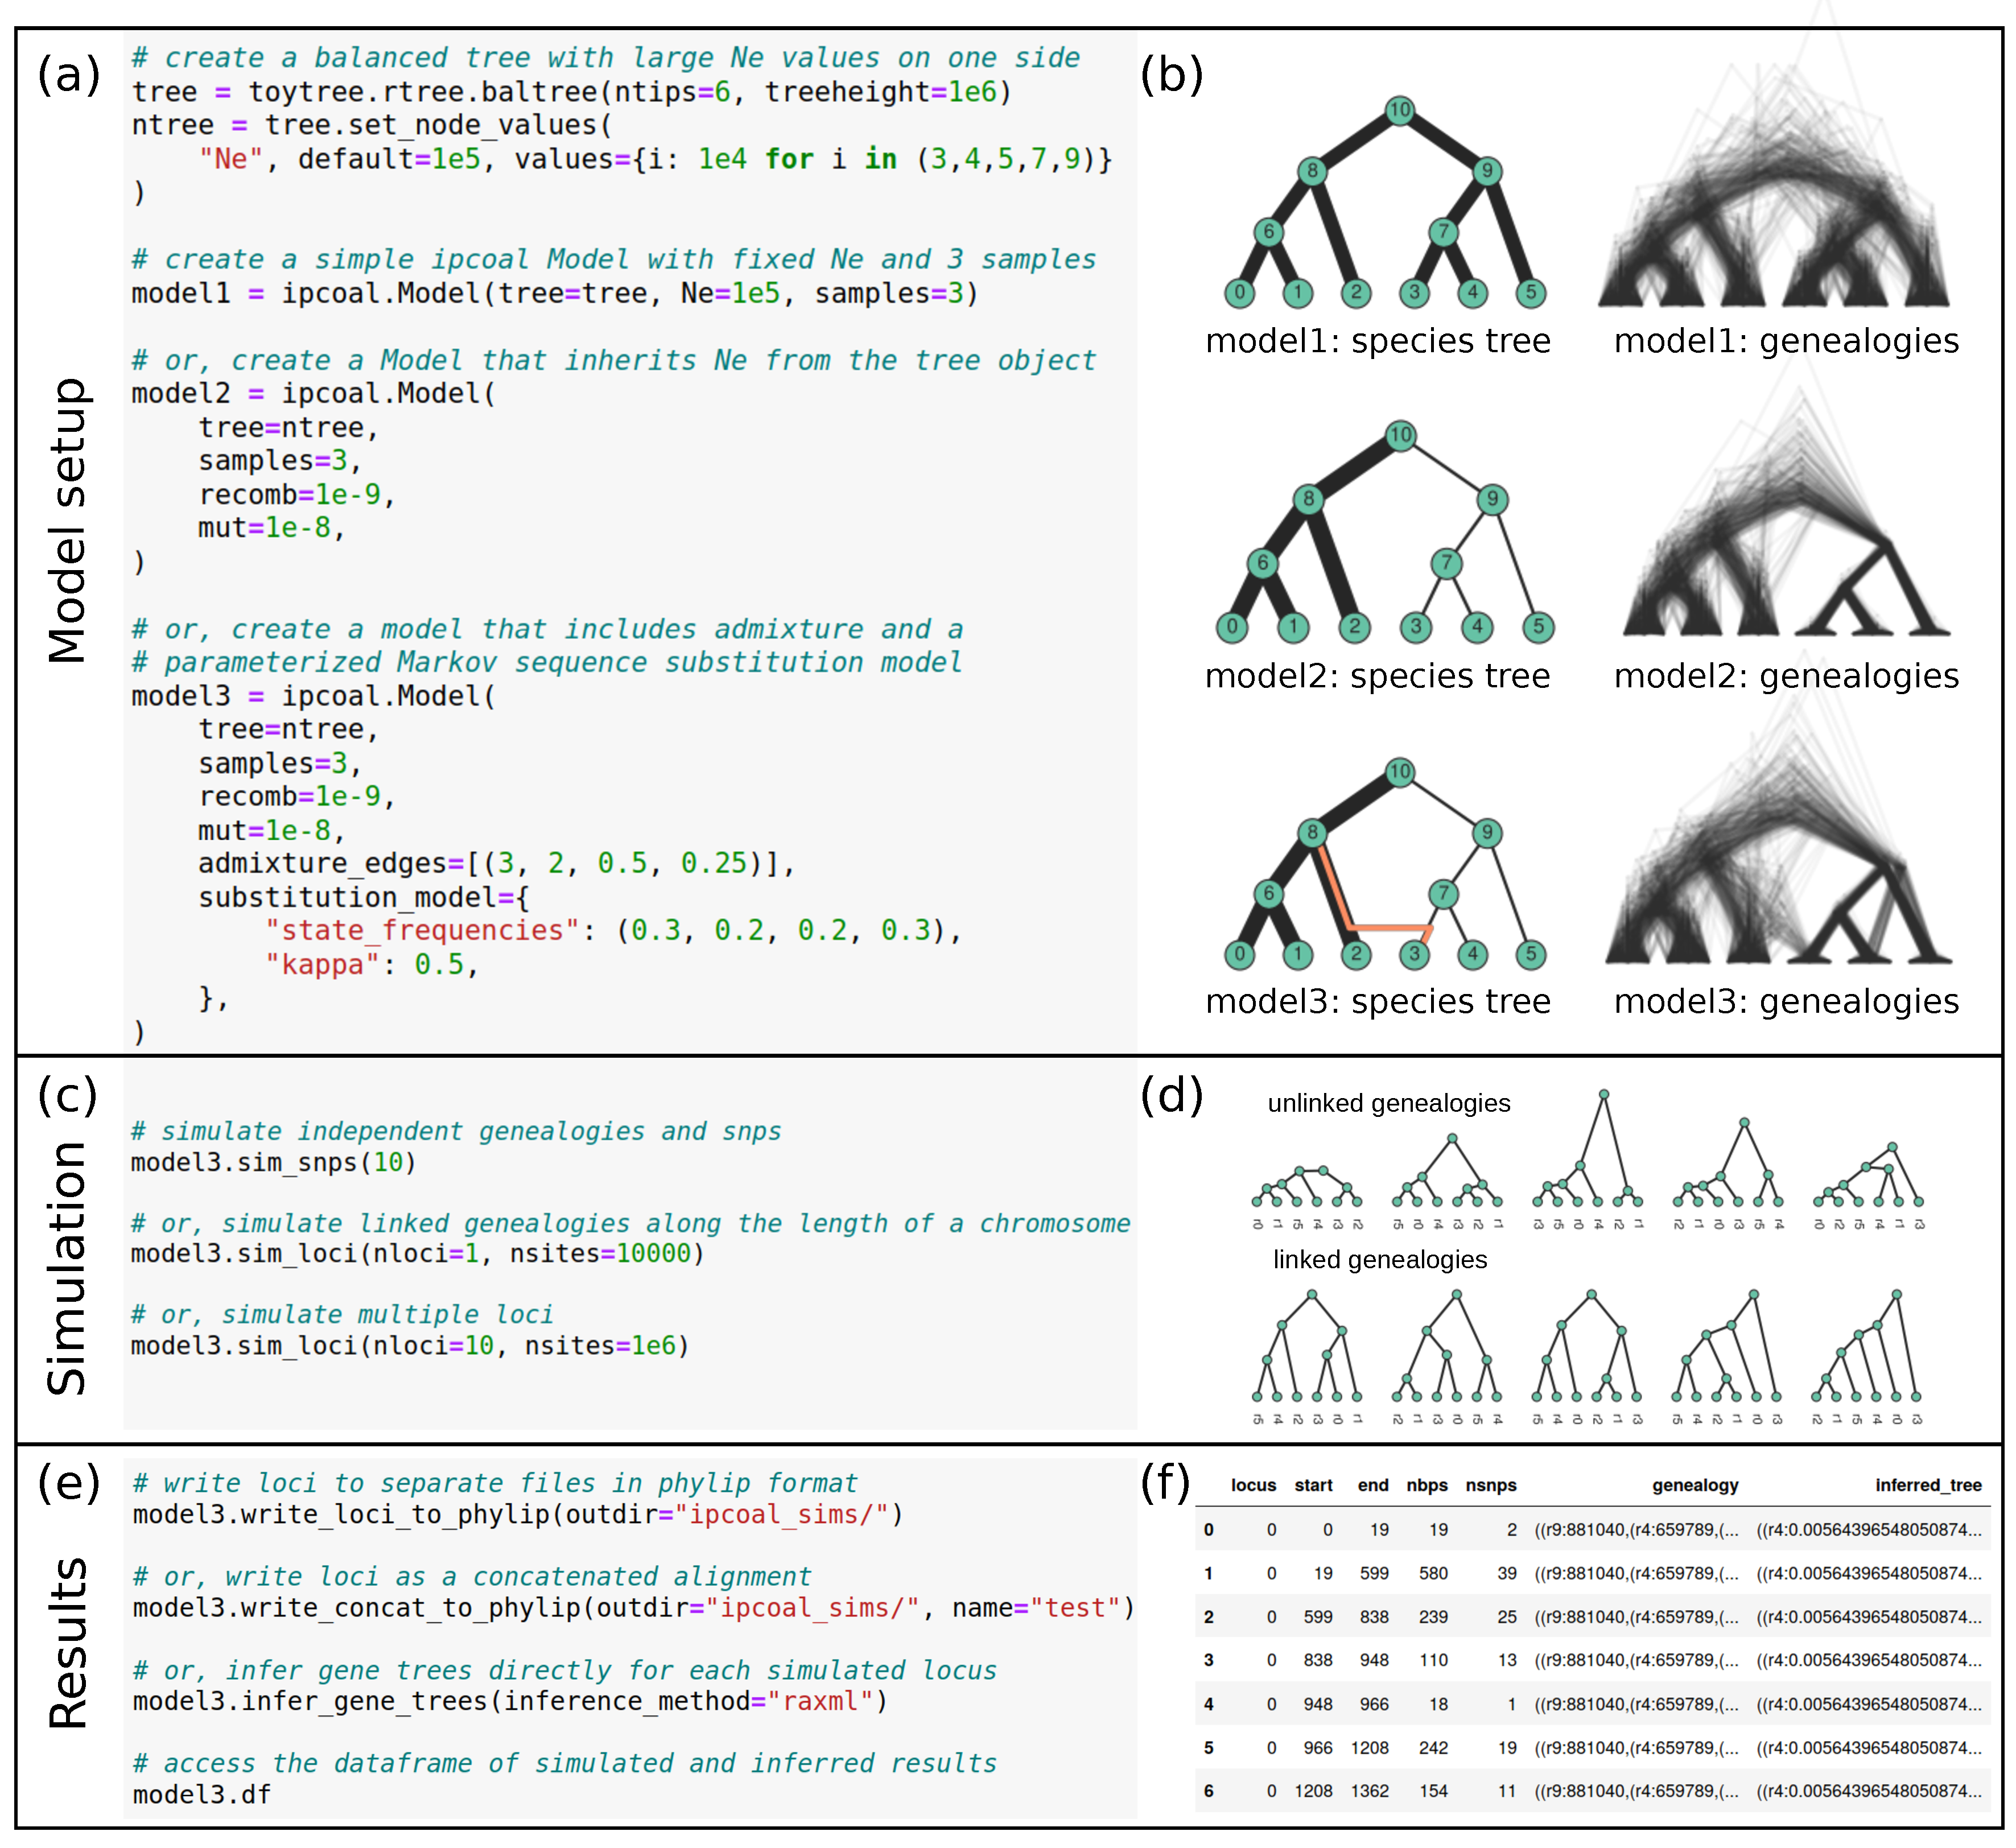
\includegraphics[width=15cm]{figures/composite.pdf}
  \caption{Simulation of coalescent genealogies and sequence data in \emph{ipcoal}. A species tree can be generated or loaded from a newick string to define population relationships in a demographic model, and a single Ne value or variable Nes can be applied to nodes by mapping values using \emph{toytree}. The Model class object of \emph{ipcoal} is used to initialize parameterized demographic and mutational models (a). Genealogical variation reflects parameters of the demographic model including Ne and admixture events, each of which can be easily visualized for validation (b). Sequence data can be simulated as unlinked SNPs (c) or as continuous loci in which recombination affects linkage among neighboring genealogies (d). Simulated sequences can be written to files (either concatenated or as separate loci) for downstream analyses, or the sequences can be used to directly infer gene trees (e). Simulated and inferred results are organized into dataframes for further analyses (f).
  % using convenience functions that call external inference programs. 
  % A dataframe summarizing simulated and inferred results  can be accessed directly for further analyses or written to a CSV file.}
  }
  \label{fig:fig1}
\end{figure}


\bibliographystyle{ecol_let}
%\bibliography{ipcoal-bioinf}  
\begin{thebibliography}{25}
\expandafter\ifx\csname natexlab\endcsname\relax\def\natexlab#1{#1}\fi

\bibitem[{Adams \& Castoe(2019)}]{adams_binning_2019}
Adams, R.H. \& Castoe, T.A. (2019).
\newblock Statistical binning leads to profound model violation due to gene
  tree error incurred by trying to avoid gene tree error.
\newblock \emph{Molecular Phylogenetics and Evolution}, 134, 164 -- 171.

\bibitem[{Adrion \emph{et~al.}(2019)Adrion, Cole, Dukler, Galloway, Gladstein,
  Gower, Kyriazis, Ragsdale, Tsambos, Baumdicker, Carlson, Cartwright,
  Durvasula, Kim, McKenzie, Messer, Noskova, Vecchyo, Racimo, Struck, Gravel,
  Gutenkunst, Lohmeuller, Ralph, Schrider, Siepel, Kelleher \&
  Kern}]{adrion_community_maintained_2019}
Adrion, J.R., Cole, C.B., Dukler, N., Galloway, J.G., Gladstein, A.L., Gower,
  G., Kyriazis, C.C., Ragsdale, A.P., Tsambos, G., Baumdicker, F., Carlson, J.,
  Cartwright, R.A., Durvasula, A., Kim, B.Y., McKenzie, P., Messer, P.W.,
  Noskova, E., Vecchyo, D.O.D., Racimo, F., Struck, T.J., Gravel, S.,
  Gutenkunst, R.N., Lohmeuller, K.E., Ralph, P.L., Schrider, D.R., Siepel, A.,
  Kelleher, J. \& Kern, A.D. (2019).
\newblock A community-maintained standard library of population genetic models.
\newblock \emph{bioRxiv}, p. 2019.12.20.885129.

\bibitem[{Beerli \& Felsenstein(2001)}]{beerli_coalescent_2001}
Beerli, P. \& Felsenstein, J. (2001).
\newblock Maximum likelihood estimation of a migration matrix and effective
  population sizes in n subpopulations by using a coalescent approach.
\newblock \emph{Proceedings of the National Academy of Sciences}, 98,
  4563--4568.

\bibitem[{Brown(2014)}]{brown_predictive_2014}
Brown, J.M. (2014).
\newblock {Predictive Approaches to Assessing the Fit of Evolutionary Models}.
\newblock \emph{Systematic Biology}, 63, 289--292.

\bibitem[{Bryant \emph{et~al.}(2012)Bryant, Bouckaert, Felsenstein, Rosenberg
  \& RoyChoudhury}]{bryant_snapp_2012}
Bryant, D., Bouckaert, R., Felsenstein, J., Rosenberg, N.A. \& RoyChoudhury, A.
  (2012).
\newblock {Inferring Species Trees Directly from Biallelic Genetic Markers:
  Bypassing Gene Trees in a Full Coalescent Analysis}.
\newblock \emph{Molecular Biology and Evolution}, 29, 1917--1932.

\bibitem[{Chifman \& Kubatko(2014)}]{chifman_quartets_2014}
Chifman, J. \& Kubatko, L. (2014).
\newblock {Quartet Inference from SNP Data Under the Coalescent Model}.
\newblock \emph{Bioinformatics}, 30, 3317--3324.

\bibitem[{Chung \& Hey(2017)}]{chung_bayesian_2017}
Chung, Y. \& Hey, J. (2017).
\newblock {Bayesian Analysis of Evolutionary Divergence with Genomic Data under
  Diverse Demographic Models}.
\newblock \emph{Molecular Biology and Evolution}, 34, 1517--1528.

\bibitem[{Degnan \& Rosenberg(2009)}]{degnan_gene_2009}
Degnan, J.H. \& Rosenberg, N.A. (2009).
\newblock Gene tree discordance, phylogenetic inference and the multispecies
  coalescent.
\newblock \emph{Trends in Ecology \& Evolution}, 24, 332--340.

\bibitem[{Eaton(2020)}]{eaton_toytree_2020}
Eaton, D.A.R. (2020).
\newblock Toytree: {A} minimalist tree visualization and manipulation library
  for {Python}.
\newblock \emph{Methods in Ecology and Evolution}, 11, 187--191.

\bibitem[{Felsenstein(1978)}]{felsenstein_parsimony_1978}
Felsenstein, J. (1978).
\newblock Cases in which parsimony or compatibility methods will be positively
  misleading.
\newblock \emph{Systematic Zoology}, 27, 401--410.

\bibitem[{Green \emph{et~al.}(2010)Green, Krause, Briggs, Maricic, Stenzel,
  Kircher, Patterson, Li, Zhai, Fritz, Hansen, Durand, Malaspinas, Jensen,
  Marques-Bonet, Alkan, Pr{\"u}fer, Meyer, Burbano, Good, Schultz, Aximu-Petri,
  Butthof, H{\"o}ber, H{\"o}ffner, Siegemund, Weihmann, Nusbaum, Lander, Russ,
  Novod, Affourtit, Egholm, Verna, Rudan, Brajkovic, Kucan, Gu{\v s}ic,
  Doronichev, Golovanova, Lalueza-Fox, de~la Rasilla, Fortea, Rosas, Schmitz,
  Johnson, Eichler, Falush, Birney, Mullikin, Slatkin, Nielsen, Kelso,
  Lachmann, Reich \& P{\"a}{\"a}bo}]{green_neandertal_2010}
Green, R.E., Krause, J., Briggs, A.W., Maricic, T., Stenzel, U., Kircher, M.,
  Patterson, N., Li, H., Zhai, W., Fritz, M.H.Y., Hansen, N.F., Durand, E.Y.,
  Malaspinas, A.S., Jensen, J.D., Marques-Bonet, T., Alkan, C., Pr{\"u}fer, K.,
  Meyer, M., Burbano, H.A., Good, J.M., Schultz, R., Aximu-Petri, A., Butthof,
  A., H{\"o}ber, B., H{\"o}ffner, B., Siegemund, M., Weihmann, A., Nusbaum, C.,
  Lander, E.S., Russ, C., Novod, N., Affourtit, J., Egholm, M., Verna, C.,
  Rudan, P., Brajkovic, D., Kucan, {\v Z}., Gu{\v s}ic, I., Doronichev, V.B.,
  Golovanova, L.V., Lalueza-Fox, C., de~la Rasilla, M., Fortea, J., Rosas, A.,
  Schmitz, R.W., Johnson, P.L.F., Eichler, E.E., Falush, D., Birney, E.,
  Mullikin, J.C., Slatkin, M., Nielsen, R., Kelso, J., Lachmann, M., Reich, D.
  \& P{\"a}{\"a}bo, S. (2010).
\newblock A draft sequence of the neandertal genome.
\newblock \emph{Science}, 328, 710--722.

\bibitem[{Gronau \emph{et~al.}(2011)Gronau, Hubisz, Gulko, Danko \&
  Siepel}]{gronau_demography_2011}
Gronau, I., Hubisz, M.J., Gulko, B., Danko, C.G. \& Siepel, A. (2011).
\newblock {Bayesian inference of ancient human demography from individual
  genome sequences}.
\newblock \emph{Nature Genetics}, 43, 1031--1035.

\bibitem[{Hudson(1983)}]{hudson_testing_1983}
Hudson, R.R. (1983).
\newblock Testing the {Constant}-{Rate} {Neutral} {Allele} {Model} with
  {Protein} {Sequence} {Data}.
\newblock \emph{Evolution}, 37, 203--217.

\bibitem[{Hudson(2002)}]{hudson_generating_2002}
Hudson, R.R. (2002).
\newblock Generating samples under a {Wright}–{Fisher} neutral model of
  genetic variation.
\newblock \emph{Bioinformatics}, 18, 337--338.

\bibitem[{Kelleher \emph{et~al.}(2016)Kelleher, Etheridge \&
  McVean}]{kelleher_efficient_2016}
Kelleher, J., Etheridge, A.M. \& McVean, G. (2016).
\newblock Efficient {Coalescent} {Simulation} and {Genealogical} {Analysis} for
  {Large} {Sample} {Sizes}.
\newblock \emph{PLOS Computational Biology}, 12, e1004842.

\bibitem[{Kim(1996)}]{kim_inconsistency_1996}
Kim, J. (1996).
\newblock {General Inconsistency Conditions for Maximum Parsimony: Effects of
  Branch Lengths and Increasing Numbers of Taxa}.
\newblock \emph{Systematic Biology}, 45, 363--374.

\bibitem[{Kingman(1982)}]{kingman_coalescent_1982}
Kingman, J.F.C. (1982).
\newblock The coalescent.
\newblock \emph{Stochastic Processes and their Applications}, 13, 235--248.

\bibitem[{Kluyver \emph{et~al.}(2016)Kluyver, Ragan-Kelley, Pérez, Granger,
  Bussonnier, Frederic, Kelley, Hamrick, Grout, Corlay, Ivanov, Avila, Abdalla,
  Willing \& al}]{kluyver_jupyter_2016}
Kluyver, T., Ragan-Kelley, B., Pérez, F., Granger, B.E., Bussonnier, M.,
  Frederic, J., Kelley, K., Hamrick, J.B., Grout, J., Corlay, S., Ivanov, P.,
  Avila, D., Abdalla, S., Willing, C. \& al, e. (2016).
\newblock Jupyter {Notebooks} - a publishing format for reproducible
  computational workflows.
\newblock In: \emph{{ELPUB}}.

\bibitem[{Knowles \& Kubatko(2011)}]{knowles_estimating_2011}
Knowles, L.L. \& Kubatko, L.S. (eds.)  (2011).
\newblock \emph{Estimating {Species} {Trees}: {Practical} and {Theoretical}
  {Aspects}}.
\newblock 1st edn.
\newblock Wiley-Blackwell.

\bibitem[{Maddison(1997)}]{maddison_gene_1997}
Maddison, W.P. (1997).
\newblock Gene {Trees} in {Species} {Trees}.
\newblock \emph{Systematic Biology}, 46, 523--536.

\bibitem[{Pamilo \& Nei(1988)}]{pamilo_relationships_1988}
Pamilo, P. \& Nei, M. (1988).
\newblock Relationships between gene trees and species trees.
\newblock \emph{Molecular Biology and Evolution}, 5, 568--583.

\bibitem[{Posada \& Crandall(2002)}]{posada_recombination_2002}
Posada, D. \& Crandall, K.A. (2002).
\newblock The effect of recombination on the accuracy of phylogeny estimation.
\newblock \emph{Journal of Molecular Evolution}, 54, 396--402.

\bibitem[{Rambaut \& Grass(1997)}]{rambaut_seqgen_1997}
Rambaut, A. \& Grass, N.C. (1997).
\newblock {Seq-Gen: an application for the Monte Carlo simulation of DNA
  sequence evolution along phylogenetic trees}.
\newblock \emph{Bioinformatics}, 13, 235--238.

\bibitem[{Reich(2018)}]{reich_who_2018}
Reich, D. (2018).
\newblock \emph{Who we are and how we got here: Ancient DNA and the new science
  of the human past}.
\newblock Oxford University Press.

\bibitem[{Schrider \& Kern(2018)}]{schrider_learning_2017}
Schrider, D.R. \& Kern, A.D. (2018).
\newblock Supervised machine learning for population genetics: A new paradigm.
\newblock \emph{Trends in Genetics}, 34, 301 -- 312.

\end{thebibliography}

\end{document}
